\documentclass[11pt,a4paper]{report}
% ==================== Packages ====================
\usepackage[a4paper,top=1in,bottom=1in,left=1.05in,right=1.05in]{geometry}
\usepackage[T1]{fontenc}
\usepackage[utf8]{inputenc}
\usepackage{charter}
\usepackage[scaled=0.92]{helvet}
\usepackage{microtype}
\usepackage{setspace}
\usepackage{titlesec}
\usepackage{fancyhdr}
\usepackage{lastpage}
\usepackage{graphicx}
\usepackage{xcolor}
\usepackage{booktabs}
\usepackage{array}
\usepackage{tabularx}
\usepackage{enumitem}
\usepackage{hyperref}
\usepackage{url}
\usepackage{tikz}
\usetikzlibrary{arrows.meta,positioning,shapes.geometric,fit,calc,backgrounds}
\usepackage{tcolorbox}
\usepackage{listings}
\usepackage{caption}
\usepackage{float}
\usepackage{amsmath}
\usepackage{amssymb}
\usepackage{ragged2e}

\graphicspath{{figures/}}

% Float placement: allow figures to pack densely instead of stranding half-pages
\setcounter{topnumber}{3}
\setcounter{bottomnumber}{2}
\setcounter{totalnumber}{4}
\renewcommand{\topfraction}{0.92}
\renewcommand{\bottomfraction}{0.75}
\renewcommand{\textfraction}{0.06}
\renewcommand{\floatpagefraction}{0.75}

% ==================== Theme ====================
\definecolor{navy}{HTML}{123A5E}
\definecolor{brandblue}{HTML}{2563EB}
\definecolor{lightblue}{HTML}{EFF5FD}
\definecolor{teal}{HTML}{0F766E}
\definecolor{lightteal}{HTML}{ECFDF5}
\definecolor{amber}{HTML}{B45309}
\definecolor{lightamber}{HTML}{FEF6E7}
\definecolor{graytext}{HTML}{55606E}
\definecolor{lightgray}{HTML}{F4F6F9}
\definecolor{dark}{HTML}{1F2937}
\definecolor{linegray}{HTML}{D3DDE8}

\hypersetup{
  colorlinks=true,
  linkcolor=navy,
  citecolor=teal,
  urlcolor=brandblue,
  pdftitle={LeadGenAI - Detailed Project Report},
  pdfauthor={Team Avengers},
  bookmarksopen=true
}

\setstretch{1.10}
\setlength{\parindent}{0pt}
\setlength{\parskip}{5pt}

\titleformat{\chapter}[display]
  {\sffamily\bfseries\color{navy}\huge}
  {\sffamily\normalsize\color{brandblue}\MakeUppercase{\chaptertitlename\ \thechapter}}
  {4pt}{\sffamily\huge}[\vspace{3pt}{\color{brandblue}\titlerule[1pt]}]
\titlespacing*{\chapter}{0pt}{-18pt}{18pt}

\titleformat{\section}{\sffamily\large\bfseries\color{navy}}{\thesection}{0.6em}{}
\titleformat{\subsection}{\sffamily\normalsize\bfseries\color{dark}}{\thesubsection}{0.6em}{}
\titlespacing*{\section}{0pt}{12pt}{4pt}
\titlespacing*{\subsection}{0pt}{9pt}{3pt}

\pagestyle{fancy}
\fancyhf{}
\lhead{\footnotesize\textcolor{graytext}{LeadGenAI --- Detailed Project Report}}
\rhead{\footnotesize\textcolor{graytext}{Team Avengers}}
\newcommand{\footcontent}{\thepage}
\cfoot{\footnotesize\textcolor{graytext}{\footcontent}}
\setlength{\headheight}{14pt}
\renewcommand{\headrulewidth}{0.4pt}
\renewcommand{\footrulewidth}{0pt}
\fancypagestyle{plain}{%
  \fancyhf{}%
  \cfoot{\footnotesize\textcolor{graytext}{\footcontent}}%
  \renewcommand{\headrulewidth}{0pt}%
  \renewcommand{\footrulewidth}{0pt}%
}

\captionsetup{font=small,labelfont={sf,bf,color=navy},skip=6pt}

\newtcolorbox{infobox}[1][]{colback=lightblue,colframe=brandblue,boxrule=0.7pt,arc=2mm,
  left=7pt,right=7pt,top=6pt,bottom=6pt,#1}
\newtcolorbox{successbox}[1][]{colback=lightteal,colframe=teal,boxrule=0.7pt,arc=2mm,
  left=7pt,right=7pt,top=6pt,bottom=6pt,#1}
\newtcolorbox{warningbox}[1][]{colback=lightamber,colframe=amber,boxrule=0.7pt,arc=2mm,
  left=7pt,right=7pt,top=6pt,bottom=6pt,#1}

\newcommand{\project}{\textbf{LeadGenAI}}

% Screenshot helper: bordered figure with caption
\newcommand{\uifig}[4]{%
\begin{figure}[htbp]
\centering
\setlength{\fboxsep}{0pt}\setlength{\fboxrule}{0.6pt}%
{\color{linegray}\fbox{\includegraphics[width=\dimexpr#2\textwidth-2\fboxrule\relax]{#1}}}
\caption{#3}\label{#4}
\end{figure}}

\lstdefinestyle{envstyle}{
  basicstyle=\ttfamily\footnotesize,
  backgroundcolor=\color{lightgray},
  frame=single,
  rulecolor=\color{linegray},
  breaklines=true,
  columns=fullflexible,
  showstringspaces=false,
  xleftmargin=4pt,xrightmargin=4pt
}

\begin{document}

% ==================== COVER ====================
\begin{titlepage}
\thispagestyle{empty}
\begin{center}
  \vspace*{0.7cm}
  {\large\bfseries\color{brandblue}PRASUNETHON 2.0 --- FINAL PROJECT SUBMISSION\par}
  \vspace{0.5cm}
  {\color{linegray}\rule{0.85\textwidth}{1.2pt}\par}
  \vspace{0.6cm}
  {\fontsize{46}{50}\selectfont\bfseries\color{navy}LeadGenAI\par}
  \vspace{0.25cm}
  {\Large\bfseries\color{dark}Intelligent B2B Lead Discovery, Calling\\and Outreach Copilot\par}
  \vspace{0.5cm}
  {\large Detailed Project Report\par}
  \vspace{0.8cm}

  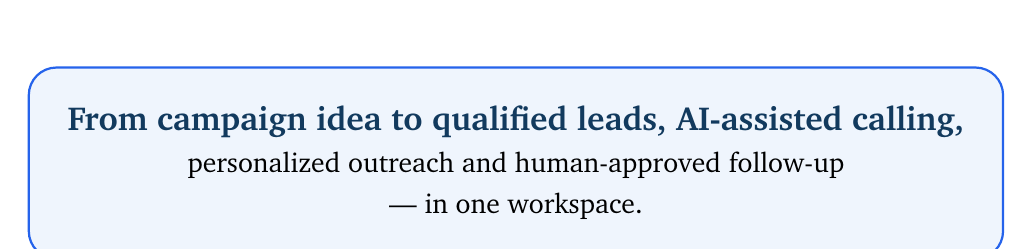
\begin{tikzpicture}
    \node[rounded corners=10pt,fill=lightblue,draw=brandblue,line width=0.8pt,
          minimum width=0.88\textwidth,inner sep=14pt,align=center] {
      \large\bfseries\color{navy}
      From campaign idea to qualified leads, AI-assisted calling,\\[3pt]
      personalized outreach and human-approved follow-up\\[3pt]
      --- in one workspace.
    };
  \end{tikzpicture}

  \vspace{0.7cm}
  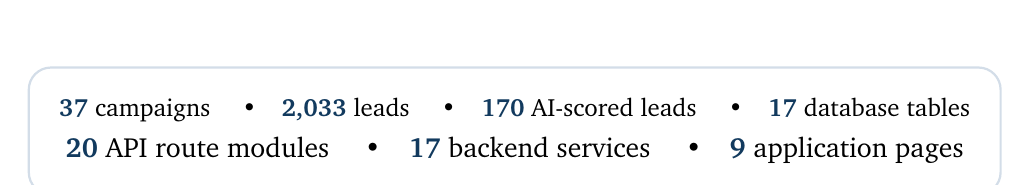
\begin{tikzpicture}
    \node[rounded corners=8pt,fill=white,draw=linegray,line width=0.8pt,
          minimum width=0.88\textwidth,inner sep=11pt,align=center] {
      \small
      \textbf{\color{navy}37} campaigns \quad\textbullet\quad
      \textbf{\color{navy}2{,}033} leads \quad\textbullet\quad
      \textbf{\color{navy}170} AI-scored leads \quad\textbullet\quad
      \textbf{\color{navy}17} database tables\\[3pt]
      \textbf{\color{navy}20} API route modules \quad\textbullet\quad
      \textbf{\color{navy}17} backend services \quad\textbullet\quad
      \textbf{\color{navy}9} application pages
    };
  \end{tikzpicture}

  \vfill
  {\large\bfseries Team Avengers\par}
  \vspace{0.2cm}
  {\normalsize Raj Gautam (Team Leader) \quad\textbullet\quad Priyanshu Kumar \quad\textbullet\quad Sampath Kumar Midde\par}
  \vspace{0.35cm}
  {\small\textbf{Live application:} \url{https://ai-lead-generation-mvp.vercel.app/}\par}
  {\small\textbf{Source repository:} \url{https://github.com/FasterThanAi/ai-lead-generation-mvp}\par}
  \vspace{0.25cm}
  {\footnotesize\color{graytext} All figures in this report are captured from the deployed application. \quad August 2026\par}
\end{center}
\end{titlepage}

% ==================== FRONT MATTER ====================
\pagenumbering{roman}

\chapter*{Declaration}
\addcontentsline{toc}{chapter}{Declaration}
This report documents \project{} as it is actually built and deployed. Every architectural claim, workflow description and numeric figure in this document was verified against the project source repository and the live application before publication, and all interface figures are screenshots of the running system rather than mock-ups.

Where a capability is implemented but constrained by an external provider plan --- most notably AI calling, which is verified against a registered test number on the current Vapi tier --- that constraint is stated explicitly at the point of description. Where a capability is deliberately deferred to future work, it appears in Chapter~\ref{ch:limits} rather than being presented as delivered. We consider this distinction to be part of the engineering, not a caveat on it.

\vspace{14pt}
{\sffamily\Large\bfseries\color{navy}Acknowledgement}
\addcontentsline{toc}{section}{Acknowledgement}
\vspace{4pt}

We thank the Prasunethon 2.0 organisers for a problem statement open enough to justify building a complete operating system rather than a single feature demonstration. The project brought together modern web engineering, generative AI, retrieval-augmented generation, workflow automation, telephony and email APIs, and --- most importantly --- the human-approval controls that make all of it safe to point at real businesses.

\tableofcontents
\listoffigures
\listoftables
\clearpage
\pagenumbering{arabic}
\renewcommand{\footcontent}{Page \thepage\ of \pageref{LastPage}}

% =====================================================
\chapter{Executive Summary}
% =====================================================
\project{} is a working AI-powered B2B lead-generation and outreach platform. It takes a sales operator from a rough campaign idea through lead discovery, contact extraction, AI research, explainable scoring, personalised email drafting, AI-assisted calling, reply classification and human-approved follow-up --- without leaving the product.

The system is deployed and in use. At the time of writing the live instance holds 37 campaigns and 2{,}033 leads, has AI-scored 170 of them, has generated 40 email drafts of which 8 were approved and 9 sent, and has captured and classified 6 replies. These are operating figures from a pilot-scale deployment, not projections.

\section{What was built}
The backend is roughly 20{,}000 lines of Python across 20 API route modules and 17 service modules, backed by a 17-table relational schema. The frontend is a nine-page React application. Behind those numbers are seven integrated subsystems: campaign management, multi-path lead discovery, public contact extraction, AI research and enrichment, a two-factor explainable scoring model, an approval-gated outreach layer covering both email and voice, and a retrieval-augmented knowledge base that grounds generated copy in the operator's own company facts.

\section{What makes it different}
Three design decisions separate \project{} from a generic AI email tool.

\textbf{Scoring is explainable and deterministic.} The final lead score is a published, reproducible function of two sub-scores --- business fit and contact confidence --- and every score carries a written reason. When the AI scorer is unavailable, a rule-based fallback produces a score using the same contract, so the pipeline degrades rather than stops. Chapter~\ref{ch:scoring} documents the model in full.

\textbf{Discovery is a boundary, not a scraper.} Automated sourcing runs through an external n8n workflow that the backend triggers by webhook and that reports results back through a public API. The scraping provider sits outside the application entirely. This keeps a rate-limited, cost-bearing, failure-prone activity out of the request path and behind a replaceable interface.

\textbf{The human approves every outbound action.} AI drafts; the operator sends. Emails, replies, follow-ups and calls all pass through an explicit approval state, and do-not-call leads are blocked server-side before any telephony request is constructed. This is enforced in code, not merely recommended in documentation.

\begin{infobox}
\textbf{Core value proposition.} \project{} connects discovery, qualification, personalised outreach, calling and follow-up into a single traceable loop, so an operator spends time on conversations rather than on preparation --- while keeping the decision to contact a real business firmly in human hands.
\end{infobox}

\uifig{01-dashboard}{0.97}{The operational dashboard of the deployed application. Reply rate is computed over a pilot-scale sample of 9 sent emails.}{fig:01-dashboard}

% =====================================================
\chapter{Problem and Objectives}
% =====================================================
\section{Background}
Business-to-business prospecting is not one task. It is a chain of loosely coupled tasks, and in most teams each link lives in a different tool. Prospects are found in business directories and maps; contact details are assembled in spreadsheets; research happens in a browser; qualification happens in someone's head; the email is written in a mail client; the call is made from a phone; the reply is triaged in an inbox; and the follow-up is remembered, or it is not.

The cost of this fragmentation is not primarily time --- it is inconsistency. Two leads with identical characteristics get different priorities depending on who looked at them and when. A promising reply gets a slower response than a lukewarm one because it arrived on a busier day. The reasoning behind a decision to pursue or drop a prospect is rarely written down, so it cannot be reviewed, improved, or handed to a colleague.

\section{Problem statement}
\begin{successbox}
\textbf{Problem.} B2B teams lose productive capacity because lead discovery, qualification, research, outreach preparation, calling and follow-up are handled in separate tools. The result is fragmented context, inconsistent prioritisation, repetitive personalisation work and dropped next actions. What is needed is a single system that finds relevant prospects, \emph{explains why they matter}, prepares outreach across channels, and keeps the decision to contact a real business under human control.
\end{successbox}

\section{Objectives}
\begin{enumerate}[leftmargin=1.4em,itemsep=2pt]
  \item Build one workspace spanning campaign definition through approved follow-up.
  \item Support several lead-entry paths --- CSV import, operator-reviewed public URLs, and automated business discovery --- feeding one common lead table.
  \item Extract contact details from public sources without depending on a paid enrichment subscription.
  \item Use generative AI for research, scoring, qualification and outreach drafting, and make its reasoning visible.
  \item Ground generated copy in the operator's own company facts through retrieval rather than fine-tuning.
  \item Support AI-assisted calling as a first-class stage of the same lead lifecycle.
  \item Require explicit human approval before any outbound email, reply or call.
  \item Keep integrations modular so providers can be replaced without rewriting the application.
\end{enumerate}

\section{Intended users}
The product is built for the lean end of the market: founders selling their own product, two-to-five person sales teams, agencies running outreach on behalf of clients, and student or research teams doing structured institutional outreach. These users share a defining constraint --- nobody has time to run six tools, and nobody has budget for enterprise sales software. The interface is therefore organised around decisions rather than subsystems, and the contact-extraction path is designed to work without a paid data subscription.

% =====================================================
\chapter{System Overview and Workflow}
% =====================================================
\section{Concept}
\project{} is designed as a closed loop. A campaign begins as a plain business goal. The platform converts it into structured context, sources leads, extracts and verifies contact details, researches each company, scores it against the campaign, prepares outreach and proposes the next safe action. Every stage writes back onto the lead record, so context accumulates rather than being re-derived.

\begin{figure}[H]
\centering
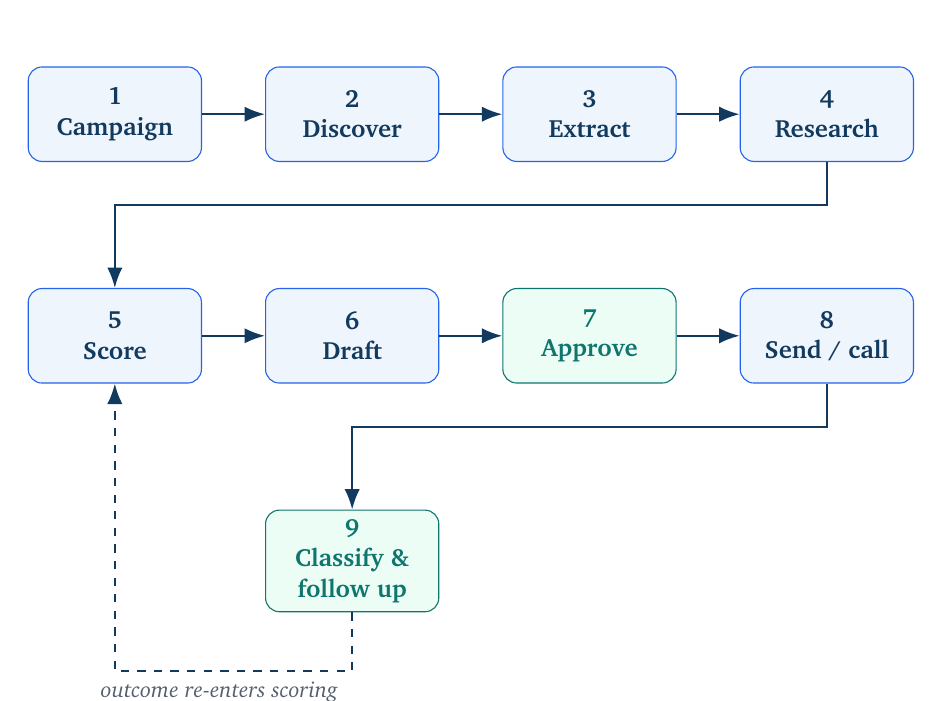
\begin{tikzpicture}[
  stage/.style={rounded corners=5pt, draw=brandblue, fill=lightblue, minimum width=2.2cm,
                minimum height=1.2cm, align=center, font=\small\bfseries, text=navy},
  gate/.style={rounded corners=5pt, draw=teal, fill=lightteal, minimum width=2.2cm,
               minimum height=1.2cm, align=center, font=\small\bfseries, text=teal},
  arrow/.style={-{Latex[length=2.6mm]}, thick, draw=navy}
]
  \node[stage] (c) {1\\Campaign};
  \node[stage,right=8mm of c] (d) {2\\Discover};
  \node[stage,right=8mm of d] (e) {3\\Extract};
  \node[stage,right=8mm of e] (r) {4\\Research};
  \node[stage,below=16mm of c] (s) {5\\Score};
  \node[stage,right=8mm of s] (o) {6\\Draft};
  \node[gate,right=8mm of o]  (a) {7\\Approve};
  \node[stage,right=8mm of a] (g) {8\\Send / call};
  \node[gate,below=16mm of o] (f) {9\\Classify \&\\follow up};
  \foreach \x/\y in {c/d,d/e,e/r,s/o,o/a,a/g}{\draw[arrow] (\x) -- (\y);}
  \draw[arrow] (r.south) -- ++(0,-0.55) -| (s.north);
  \draw[arrow] (g.south) -- ++(0,-0.55) -| (f.north);
  \draw[arrow,dashed] (f.south) -- ++(0,-0.75)
        -| node[pos=0.28,below,font=\footnotesize\itshape,text=graytext]{outcome re-enters scoring} (s.south);
\end{tikzpicture}
\caption{The \project{} operating loop. Stages 7 and 9 (green) are human-controlled checkpoints; every other stage is AI- or automation-driven. Outcomes feed back into scoring rather than terminating the lead.}
\label{fig:loop}
\end{figure}

\section{The human-in-the-loop principle}
The most important structural decision is where the loop is cut. AI performs all preparation --- searching, extracting, researching, scoring, drafting. The operator performs every consequential external action --- sending an email, placing a call, replying to a prospect. The boundary is enforced in the backend rather than observed by convention: drafts carry an approval state, sending endpoints reject unapproved drafts, and telephony requests are refused for do-not-call leads.

\begin{infobox}
\textbf{Control loop:} Draft $\rightarrow$ Review $\rightarrow$ Approve $\rightarrow$ Send or Call $\rightarrow$ Log outcome $\rightarrow$ Generate next action.
\end{infobox}

This design costs throughput and buys trust. A fully autonomous version would send more email per hour --- and on the day a prompt regressed or a scraper returned malformed data, it would send that email to the wrong people and nobody would know until the replies arrived. For a tool contacting real businesses under a real sender identity, that trade is not close.

\section{Context accumulation}
A subtler consequence of the loop in Figure~\ref{fig:loop} is that no stage re-derives what an earlier stage already established. Discovery writes the source and the raw business record; extraction writes the address and the method that found it; research writes the profile and its confidence; scoring writes the score, its components and its written reason; drafting writes the copy and the knowledge it drew on; sending, calling and classification each write their outcome. All of it lands on the same lead row.

This matters for three reasons. It is cheaper --- research and scoring are the expensive model calls, and they run once per lead rather than once per action taken on that lead. It is auditable --- an operator asking six weeks later why a particular company was contacted can read the reasoning that existed at the time rather than reconstructing it. And it is what makes the feedback edge in Figure~\ref{fig:loop} possible at all: an outcome can only adjust a lead's priority if the evidence behind that priority is still on the record.

The alternative --- recomputing context at each step from whatever the model can infer in the moment --- produces a system whose behaviour is not reproducible from one run to the next. For a tool whose output is a decision to contact a real business, reproducibility is not a nicety.

% =====================================================
\chapter{System Architecture}
% =====================================================
\section{Layered architecture}
The application separates into four layers with explicit boundaries. The browser holds no credentials and talks only to the backend. The backend owns all business logic, orchestration and secrets. Persistence is a single relational store. External providers --- the language model, mail, telephony, automation --- are reached only through backend service modules, each of which can be replaced without touching the layers above it.

\begin{figure}[H]
\centering
\resizebox{0.97\textwidth}{!}{%
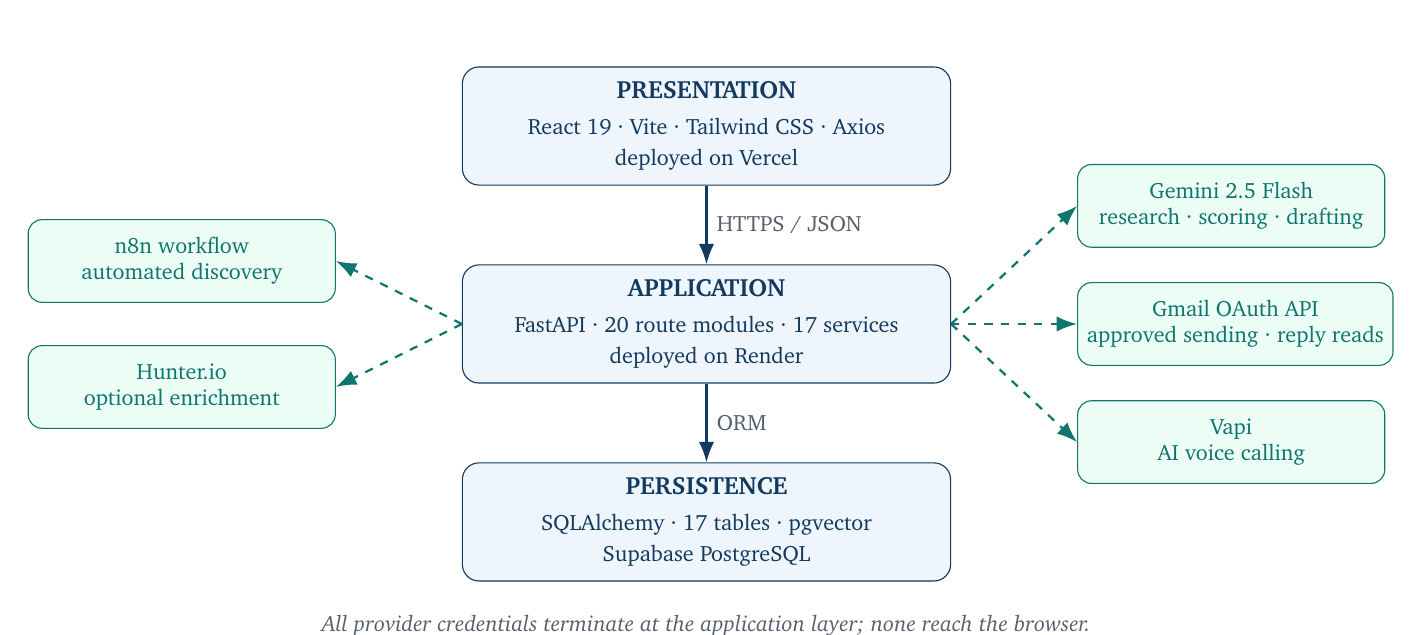
\begin{tikzpicture}[
  layer/.style={rounded corners=6pt, draw=navy, fill=lightblue, minimum width=6.2cm,
                minimum height=1.5cm, align=center, font=\small\bfseries, text=navy},
  ext/.style={rounded corners=5pt, draw=teal, fill=lightteal, minimum width=3.9cm,
              minimum height=1.05cm, align=center, font=\footnotesize, text=teal},
  arr/.style={-{Latex[length=2.6mm]}, thick, draw=navy},
  arrx/.style={-{Latex[length=2.6mm]}, thick, draw=teal, dashed}
]
  \node[layer] (ui) {PRESENTATION\\[2pt]\footnotesize\mdseries React 19 · Vite · Tailwind CSS · Axios\\\footnotesize\mdseries deployed on Vercel};
  \node[layer,below=10mm of ui] (api) {APPLICATION\\[2pt]\footnotesize\mdseries FastAPI · 20 route modules · 17 services\\\footnotesize\mdseries deployed on Render};
  \node[layer,below=10mm of api] (db) {PERSISTENCE\\[2pt]\footnotesize\mdseries SQLAlchemy · 17 tables · pgvector\\\footnotesize\mdseries Supabase PostgreSQL};

  \node[ext,right=16mm of api,yshift=15mm] (gem) {Gemini 2.5 Flash\\research · scoring · drafting};
  \node[ext,right=16mm of api]             (gml) {Gmail OAuth API\\approved sending · reply reads};
  \node[ext,right=16mm of api,yshift=-15mm](vapi){Vapi\\AI voice calling};
  \node[ext,left=16mm of api,yshift=8mm]   (n8n) {n8n workflow\\automated discovery};
  \node[ext,left=16mm of api,yshift=-8mm]  (hunt){Hunter.io\\optional enrichment};

  \draw[arr] (ui) -- node[right,font=\footnotesize,text=graytext]{HTTPS / JSON} (api);
  \draw[arr] (api) -- node[right,font=\footnotesize,text=graytext]{ORM} (db);
  \draw[arrx] (api.east) -- (gem.west);
  \draw[arrx] (api.east) -- (gml.west);
  \draw[arrx] (api.east) -- (vapi.west);
  \draw[arrx] (api.west) -- (n8n.east);
  \draw[arrx] (api.west) -- (hunt.east);
  \node[font=\footnotesize\itshape,text=graytext,below=3mm of db] {All provider credentials terminate at the application layer; none reach the browser.};
\end{tikzpicture}}
\caption{Layered architecture. Solid arrows are internal data flow; dashed arrows are outbound integrations, each isolated behind a replaceable service module.}
\label{fig:arch}
\end{figure}

\section{The automation boundary}
\label{sec:n8n}
Automated lead sourcing is the one part of the system that deliberately lives outside the application. When an operator triggers the Lead Agent, the backend generates search queries from campaign context and calls an n8n webhook. From there the workflow --- not the backend --- calls the Apify Google Maps actor, normalises the results, and posts leads back into the application through its public lead-creation endpoint.

\begin{warningbox}
\textbf{Note for reviewers.} The Apify scraping provider does not appear anywhere in the application source tree, and this is intentional. It is invoked from the n8n workflow shown in Figure~\ref{fig:n8ncanvas}. Figure~\ref{fig:n8narch} documents the full trigger-to-callback path across that boundary.
\end{warningbox}

Three properties motivated this split. Scraping is slow and rate-limited, so keeping it out of the HTTP request path prevents a discovery run from occupying a backend worker for minutes. Scraping is metered --- roughly \$0.004 per lead --- so isolating it makes the cost visible and capped at the point of use rather than buried in application logic. And scraping providers change; because the contract between the two sides is a webhook in and a REST call back, the provider can be swapped without a backend deployment.

\begin{figure}[H]
\centering
\resizebox{\textwidth}{!}{%
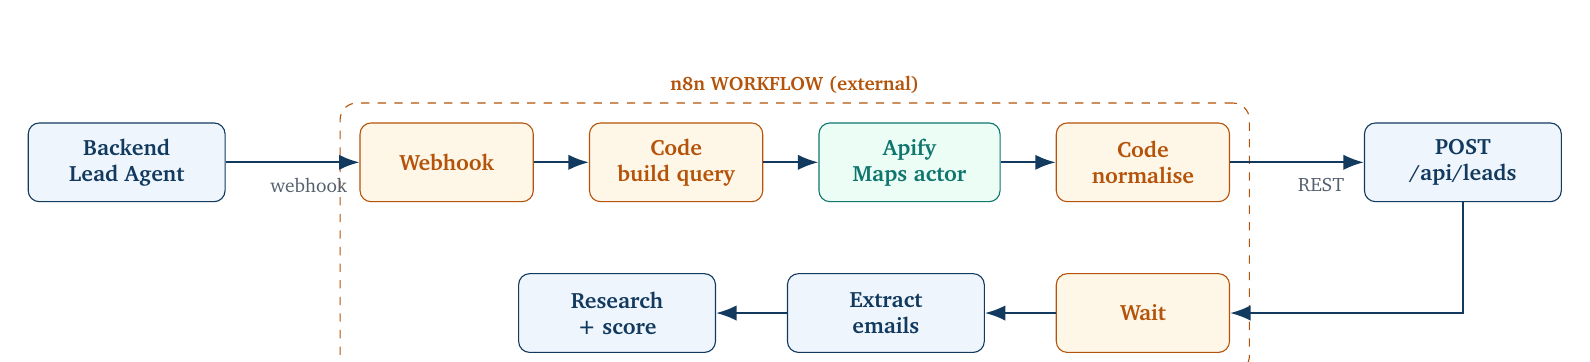
\begin{tikzpicture}[
  app/.style={rounded corners=4pt, draw=navy, fill=lightblue, minimum width=2.5cm,
              minimum height=1.0cm, align=center, font=\footnotesize\bfseries, text=navy},
  n8/.style={rounded corners=4pt, draw=amber, fill=lightamber, minimum width=2.2cm,
             minimum height=1.0cm, align=center, font=\footnotesize\bfseries, text=amber},
  extn/.style={rounded corners=4pt, draw=teal, fill=lightteal, minimum width=2.3cm,
               minimum height=1.0cm, align=center, font=\footnotesize\bfseries, text=teal},
  arr/.style={-{Latex[length=2.6mm]}, thick, draw=navy}
]
  \node[app] (be) {Backend\\Lead Agent};
  \node[n8,right=17mm of be]  (wh)  {Webhook};
  \node[n8,right=7mm of wh]  (cd)  {Code\\build query};
  \node[extn,right=7mm of cd](ap)  {Apify\\Maps actor};
  \node[n8,right=7mm of ap]  (cd1) {Code\\normalise};
  \node[app,right=17mm of cd1](cr)  {POST\\/api/leads};
  \node[n8,below=9mm of cd1] (wt)  {Wait};
  \node[app,left=9mm of wt]  (ex)  {Extract\\emails};
  \node[app,left=9mm of ex]  (sc)  {Research\\+ score};

  \draw[arr] (be) -- node[pos=0.62,below,font=\scriptsize,text=graytext,yshift=-2pt]{webhook} (wh);
  \draw[arr] (wh) -- (cd);
  \draw[arr] (cd) -- (ap);
  \draw[arr] (ap) -- (cd1);
  \draw[arr] (cd1) -- node[pos=0.68,below,font=\scriptsize,text=graytext,yshift=-2pt]{REST} (cr);
  \draw[arr] (cr.south) |- (wt.east);
  \draw[arr] (wt) -- (ex);
  \draw[arr] (ex) -- (sc);

  \begin{scope}[on background layer]
    \node[draw=amber,dashed,rounded corners=6pt,inner sep=7pt,
          fit=(wh)(cd)(cd1)(wt),label={[font=\scriptsize\bfseries,text=amber]above:n8n WORKFLOW (external)}] {};
  \end{scope}
\end{tikzpicture}}
\caption{The Lead Agent automation boundary. The backend triggers the workflow and receives leads back through its own public API; the scraping provider is reached only from inside n8n.}
\label{fig:n8narch}
\end{figure}

\uifig{14-n8n}{0.99}{The deployed n8n workflow, shown as evidence that the boundary in Figure~\ref{fig:n8narch} is real and active. The readable form of the same chain is Figure~\ref{fig:n8narch}.}{fig:n8ncanvas}

\section{Technology stack}
\begin{table}[H]
\centering
\caption{Technology stack and the role each component plays}
\small
\begin{tabularx}{\textwidth}{>{\bfseries\raggedright\arraybackslash}p{2.3cm} >{\raggedright\arraybackslash}p{5.0cm} X}
\toprule
Layer & Technology & Role \\
\midrule
Frontend & React 19, Vite, Tailwind CSS 4, Axios, Recharts & Nine-page operator interface, charts, API consumption \\
Backend & FastAPI, SQLAlchemy & Workflow orchestration, AI prompting, integration control \\
Database & Supabase PostgreSQL + pgvector & Campaigns, leads, drafts, calls, knowledge, embeddings \\
Model & Gemini 2.5 Flash & Query generation, research, scoring, drafting, classification \\
Embeddings & \texttt{gemini-embedding-001} (3072-d) & Semantic retrieval over the knowledge base \\
Automation & n8n + Apify Maps actor & Automated business discovery (see \S\ref{sec:n8n}) \\
Email & Gmail OAuth API & Approved sending and reply retrieval \\
Voice & Vapi & AI call placement, transcripts, outcomes \\
Enrichment & Hunter.io & Optional fallback when public extraction finds nothing \\
Hosting & Vercel, Render, Supabase & Frontend, backend and managed database \\
\bottomrule
\end{tabularx}
\end{table}

% =====================================================
\chapter{Product Walkthrough}
% =====================================================
This chapter follows a single lead through the system, using screenshots from the deployed application. The worked example is a live campaign targeting mechanical and industrial manufacturers in the Kanpur region.

\section{Campaigns}
A campaign is the context object that every downstream stage reads. It captures industry, location, target role and the offer being made. Because the AI stages consume these fields directly, campaign quality determines output quality: a vague offer produces vague research and generic email copy.

\uifig{02-campaigns}{0.97}{The campaign list. Each campaign carries its industry, location and target role, and can launch a discovery job directly.}{fig:02-campaigns}

\uifig{03-campaign-summary}{0.9}{Campaign context for the worked example. The offer field is deliberately verbose --- it is injected into research, scoring and drafting prompts, so specificity here propagates through the whole pipeline.}{fig:03-campaign-summary}

\section{Lead discovery}
Three entry paths feed one lead table: CSV upload for existing lists, operator-reviewed public URLs for targeted sourcing, and the automated Lead Agent for volume. The discovery form makes the boundaries explicit in the interface itself --- it states that search-query mode returns copyable queries rather than scraping search results, and that login-gated pages and LinkedIn are out of scope.

\uifig{04-discovery-job}{0.93}{Creating a discovery job. The interface states the sourcing policy at the point of use rather than burying it in documentation.}{fig:04-discovery-job}

\uifig{05-lead-agent}{0.9}{Lead Agent configuration and discovery statistics. Provider cost is shown before the run is triggered; 118 leads were sourced for this campaign, all with an email recovered.}{fig:05-lead-agent}

\section{AI research and enrichment}
Once a lead exists, the research stage fetches a limited number of its public pages and combines them with campaign context to produce a structured profile: summary, business type, likely pain points, use-case fit, outreach angle, risk flags and a confidence value.

The example in Figure~\ref{fig:research} is instructive precisely because it is a weak result. The company's website text was unavailable, so the model had only basic lead fields to work with --- and it says so. The summary records that research data was limited, the pain-point field explicitly declines to assert a specific problem, and the risk-flag field notes both that the address is generic and that the analysis used CSV and campaign data only.

\uifig{06-ai-research}{0.99}{An AI research profile for a lead whose website could not be read. The model reports its own evidence gap rather than inventing a business problem.}{fig:research}

This behaviour is deliberate. A research layer that always returns confident-sounding output is worse than useless in a sales context, because the operator cannot tell the well-evidenced leads from the guesses. Propagating the uncertainty into the record --- and then into the contact-confidence component of the score --- means a thin research result lowers the lead's priority automatically.

\section{Outreach drafting and approval}
Draft generation combines lead fields, campaign context, research output, score signals and any relevant retrieved company knowledge. The draft is created in an unsent state; the operator approves, edits or rejects it.

\uifig{08-email-draft}{0.93}{A generated cold email with its approval controls. The score breakdown is shown inline (Final 65 = Fit 60, Contact 80) so the operator can weigh the draft against the lead's qualification before sending.}{fig:08-email-draft}

\section{Reply classification}
Replies retrieved from Gmail are classified for intent, sentiment and priority, summarised, and mapped to a recommended next action. Classification never triggers a send; it produces a recommendation and, on request, a response draft that re-enters the same approval gate.

\uifig{10-replies}{0.93}{Classified replies. Each carries an intent label, sentiment, priority and a specific recommended next action rather than a generic status.}{fig:10-replies}

\section{Knowledge base and retrieval}
The knowledge layer stores company facts --- product detail, pricing guidance, FAQ content, demo notes, objection handling --- as searchable chunks. Documents in PDF, DOCX, TXT and Markdown are ingested and split automatically. Retrieval is hybrid: semantic search over 3072-dimensional embeddings via pgvector, with keyword search as both a complement and a fallback when embeddings are unavailable.

\uifig{11-knowledge}{0.99}{The knowledge base with ingested document chunks and hybrid retrieval controls. Retrieved facts are injected into the generation context; the language model is not fine-tuned on this content.}{fig:11-knowledge}

\section{AI calling}
Calling is a stage of the same lead lifecycle rather than a separate tool. The operator selects a qualified lead, generates a context-aware call script, and places the call through Vapi. Provider status, outcome, sentiment, transcript, summary and recording URL are written back to the lead, and an interested outcome can generate a follow-up email draft --- which is a draft, subject to the same approval gate as any other outbound message.

\uifig{12-calls}{0.9}{The calling console. Vapi is enabled with an assistant and phone number; calls are placed to a registered test number on the current provider tier.}{fig:12-calls}

\begin{warningbox}
\textbf{Provider constraint.} AI calling is fully implemented and verified end to end, but the current Vapi plan permits outbound calls only to a registered test number. The call path, script generation, outcome capture and follow-up generation are all exercised by that route; lifting the restriction is a billing change, not an engineering one.
\end{warningbox}

\section{Campaign generation and settings}
The Opportunities module inverts the usual starting point: instead of requiring a structured campaign up front, it accepts a rough goal in plain language and generates a reviewable strategy --- audience, pain points, value proposition, outreach angle, search keywords --- which can then be promoted into a real campaign or a discovery job.

\uifig{13-opportunities}{0.95}{The Opportunity generator turns an informal goal into a reviewable campaign strategy before any campaign or discovery job is created.}{fig:13-opportunities}

\uifig{09-settings}{0.9}{Integration status. The page states the sending policy next to the connection state --- Gmail sending is limited to approved drafts and follow-ups.}{fig:09-settings}

% =====================================================
\chapter{The Lead Scoring Model}
\label{ch:scoring}
% =====================================================
Scoring is the component that most determines whether the product is useful, because everything downstream --- which leads get researched, drafted, called and followed up --- is ordered by it. It is therefore the component that most needs to be explainable.

\section{Score composition}
The final score is a fixed, published combination of two independently computed sub-scores:
\[
S_{\text{final}} \;=\; \operatorname{round}\bigl(0.75 \cdot S_{\text{fit}} \;+\; 0.25 \cdot S_{\text{contact}}\bigr)
\]
where $S_{\text{fit}} \in [0,100]$ measures how well the business matches the campaign, and $S_{\text{contact}} \in [0,100]$ measures how likely the stored contact details are to reach a decision-maker.

Separating the two is what makes the score actionable. A single blended number cannot distinguish \emph{this is the wrong company} from \emph{this is the right company but we have the wrong email address} --- yet those two situations call for opposite responses. The first means drop the lead; the second means find a better contact. The 75/25 weighting encodes a deliberate judgement: business fit is the harder problem and the more durable signal, while contact quality is comparatively cheap to improve once a good-fit company has been identified.

\section{Business fit}
Fit is assembled from campaign-relative evidence: industry match, graded from direct through related to adjacent; role match against the campaign's target role, with decision-maker and manager roles scored separately; geographic proximity to the campaign location; offer relevance; and a research-confidence adjustment that rewards well-evidenced profiles and penalises those the research stage flagged as a poor use-case fit.

\section{Contact confidence}
Contact confidence begins at a floor and rises with the quality of what is known, with hard ceilings applied for categories of address that are structurally unreliable.

\begin{table}[H]
\centering
\caption{Contact-confidence ceilings by address category}
\small
\begin{tabularx}{\textwidth}{>{\raggedright\arraybackslash}p{5.6cm} >{\centering\arraybackslash}p{1.9cm} X}
\toprule
\textbf{Address category} & \textbf{Ceiling} & \textbf{Rationale} \\
\midrule
No email on record & 25 & Nothing to send to \\
Student or institutional domain & 45 & Rarely a purchasing decision-maker \\
Personal domain (Gmail, etc.) & 55 & Usable, but not a verified business contact \\
Domain matches the company site & 100 & Strongest available evidence of a real business contact \\
\bottomrule
\end{tabularx}
\end{table}

Extraction method feeds the same judgement. An address scraped directly from a company page is treated as strong evidence; a pattern-guessed address confirmed by SMTP probe stronger still; one confirmed only by an MX-record lookup materially weaker; and an unverified pattern guess weaker again.

\begin{table}[H]
\centering
\caption{Email confidence by verification method}
\small
\begin{tabularx}{\textwidth}{>{\raggedright\arraybackslash}p{5.6cm} >{\centering\arraybackslash}p{1.9cm} X}
\toprule
\textbf{Method} & \textbf{Confidence} & \textbf{Meaning} \\
\midrule
Pattern verified (SMTP) & 95 & Mailbox accepted the recipient at the SMTP layer \\
Direct extraction & 90 & Address published on the company's own pages \\
MX record only & 75 & Domain accepts mail; mailbox unconfirmed \\
Pattern fallback & 60 & Structurally plausible guess, unverified \\
\bottomrule
\end{tabularx}
\end{table}

\section{Priority and qualification bands}
The final score maps onto two independent labels --- an operational priority and a sales-temperature qualification.

\begin{table}[H]
\centering
\caption{Score bands}
\small
\begin{tabularx}{\textwidth}{p{3.2cm} p{3.6cm} X}
\toprule
\textbf{Final score} & \textbf{Priority} & \textbf{Qualification} \\
\midrule
80 -- 100 & High & Hot \\
60 -- 79 & Medium & Warm \\
50 -- 59 & Medium & Cold \\
30 -- 49 & Low & Cold \\
0 -- 29 & Low & Not relevant \\
\bottomrule
\end{tabularx}
\end{table}

\section{A worked example}
Figure~\ref{fig:score} shows the model separating fit from reachability on a real lead. The company is a strong campaign match and scores 95 on fit. But the only email recovered for it is \texttt{press@google.com} --- an address whose domain does not match the company, recovered from a Maps listing rather than the company's own site. Contact confidence is accordingly 25.

\[
S_{\text{final}} = \operatorname{round}(0.75 \times 95 + 0.25 \times 25) = \operatorname{round}(77.5) = 78
\]

\uifig{07-lead-score}{0.99}{Fit and contact confidence scored independently. A high-fit company with an unusable contact address lands at 78 rather than in the high-priority band --- and the interface offers \emph{Extract Email} and \emph{Research Lead} as the corrective actions.}{fig:score}

A blended scorer would have returned a single number in the seventies and left the operator to guess why. Here the diagnosis is immediate: the company is worth pursuing, the contact route is not, and the fix is to find a better address rather than to drop the lead.

The weighting also explains the shape of the boundary cases. Because fit carries three quarters of the weight, a poor-fit company cannot be rescued by an excellent contact address --- a fit of 20 with a perfect contact score still lands at 35, deep in the low band. The reverse is deliberately not true: a strong-fit company with no email at all still reaches 71, comfortably inside the medium band, because the system's judgement is that finding a better address for a well-matched business is ordinary sales work, while finding a better business for a well-known address is not a task at all.

\section{What the score is not}
It is worth being precise about the claim. The final score is not a probability of conversion, and the system does not present it as one. It is a ranking signal over evidence the platform actually holds, calibrated so that the top of the list is where an operator's next hour is best spent. Two consequences follow. A score of 78 does not mean a 78\% chance of anything; and scores are only comparable within a campaign, because fit is computed relative to that campaign's industry, role and offer.

The honest limitation is that the model has never been validated against conversion outcomes, because the pilot has not generated enough of them --- 6 classified replies is not a training signal. Outcome-weighted scoring is on the roadmap in Chapter~\ref{ch:limits} for exactly this reason. Until that data exists, the defensible claim is the one made here: the score is explainable, reproducible, and orders leads by evidence rather than by order of arrival.

\section{Deterministic fallback}
When the AI scorer is unavailable --- provider outage, rate limit, malformed response --- a rule-based fallback computes a score from the same evidence using explicit point allocations, and returns it through the same contract. The pipeline degrades in quality rather than halting, and because both paths emit the same fields, nothing downstream needs to know which one produced a given score.

% =====================================================
\chapter{Data Model and API Surface}
% =====================================================
\section{Core entities}
The schema comprises 17 tables. The lead record is the hub: campaigns own leads, and research, scoring, drafts, calls and follow-ups all attach to the lead, so context accumulates on one object through the lifecycle. Asynchronous work --- email extraction, research, scoring, discovery --- is tracked in dedicated job tables so that progress survives a page reload and partial failures remain visible.

\begin{figure}[H]
\centering
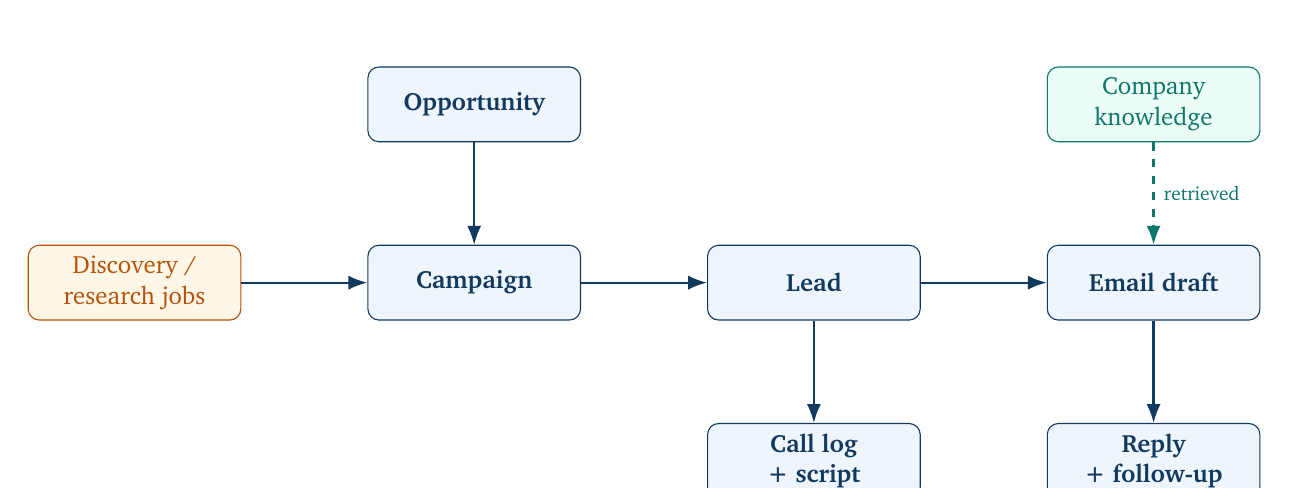
\begin{tikzpicture}[
  ent/.style={rectangle, rounded corners=4pt, draw=navy, fill=lightblue, minimum width=2.7cm,
              minimum height=0.95cm, align=center, font=\small\bfseries, text=navy},
  job/.style={rectangle, rounded corners=4pt, draw=amber, fill=lightamber, minimum width=2.7cm,
              minimum height=0.95cm, align=center, font=\small, text=amber},
  kn/.style={rectangle, rounded corners=4pt, draw=teal, fill=lightteal, minimum width=2.7cm,
             minimum height=0.95cm, align=center, font=\small, text=teal},
  rel/.style={-{Latex[length=2.4mm]}, thick, draw=navy},
  relk/.style={-{Latex[length=2.4mm]}, thick, draw=teal, dashed}
]
  \node[ent] (camp) {Campaign};
  \node[ent,right=16mm of camp] (lead) {Lead};
  \node[ent,right=16mm of lead] (draft) {Email draft};
  \node[job,left=16mm of camp]  (jobs) {Discovery /\\research jobs};
  \node[ent,above=13mm of camp] (opp)  {Opportunity};
  \node[kn,above=13mm of draft] (know) {Company\\knowledge};
  \node[ent,below=13mm of lead] (call) {Call log\\+ script};
  \node[ent,below=13mm of draft](reply){Reply\\+ follow-up};

  \draw[rel] (opp)  -- (camp);
  \draw[rel] (jobs) -- (camp);
  \draw[rel] (camp) -- (lead);
  \draw[rel] (lead) -- (draft);
  \draw[rel] (lead) -- (call);
  \draw[rel] (draft) -- (reply);
  \draw[relk] (know) -- node[right,font=\scriptsize,text=teal]{retrieved} (draft);
\end{tikzpicture}}
\caption{Simplified logical data model. The lead is the hub, accumulating research, scoring, drafts and call records through its lifecycle. Company knowledge (green) is global and retrieved into generation rather than owned by any single lead.}
\end{figure}

\section{API surface}
\begin{table}[H]
\centering
\caption{Backend API areas across 20 route modules}
\small
\begin{tabularx}{\textwidth}{>{\bfseries\raggedright\arraybackslash}p{4.2cm} X}
\toprule
Area & Responsibility \\
\midrule
Campaigns, Opportunities & Campaign context, AI-generated campaign strategies \\
Leads, Discovery & Upload, create, export, discovery jobs, source review \\
Lead Agent & Trigger n8n automation, report campaign lead status \\
AI, Lead scoring & Research, enrichment, scoring, rescoring \\
Emails, Followups & Draft generation, approval state, send, status \\
Gmail, Replies & OAuth, approved sending, reply retrieval and classification \\
Calls & Script generation, call placement, outcome and transcript capture \\
Knowledge & Document ingestion, chunking, hybrid retrieval \\
Dashboard, Analytics & Operational statistics, service status, health checks \\
Hunter, Apollo & Optional third-party enrichment \\
\bottomrule
\end{tabularx}
\end{table}

% =====================================================
\chapter{Security, Safety and Governance}
% =====================================================
\section{Approval gating}
The primary safety control is architectural. Emails, replies and follow-ups exist first as drafts; sending endpoints reject anything not in an approved state. The Lead Agent creates leads but never initiates contact. This is stated to the operator in the interface itself, on the settings page, so the guarantee is visible rather than implicit.

\section{Do-not-call enforcement}
Leads flagged do-not-call are rejected server-side before a telephony request is constructed. Placing the check in the backend rather than the interface means it holds regardless of how the endpoint is reached.

\section{Credential isolation}
All provider credentials --- language model, mail, telephony, enrichment, automation --- are held by the backend and loaded from the deployment environment. The frontend build carries only the public API base URL. No secret is reachable from the browser, and the calling console states this explicitly.

\section{Sourcing policy}
Discovery operates on operator-reviewed public URLs and public business listings. Login-gated pages, CAPTCHA-protected pages and automated LinkedIn scraping are excluded, and the constraint is printed on the discovery form rather than left to documentation. Discovered contacts remain pending until an operator reviews and imports them.

\section{Known gaps}
\label{sec:gaps}
Two limitations are material enough to state plainly rather than leave for the reader to find.

\textbf{The API has no authentication layer.} Every endpoint is currently unauthenticated. In the present single-operator deployment this is contained, but it is the blocking item before any multi-user or public exposure. The remediation is well-defined --- token authentication, per-user campaign and lead ownership, and role-based access control --- and heads the roadmap in Chapter~\ref{ch:limits}.

\textbf{SMTP verification degrades in cloud deployment.} The strongest verification tier probes recipient acceptance on port 25, which most cloud hosts block outbound. In production the check fails closed and confidence caps at the MX tier (75) rather than the verified tier (95). Scores stay correct and conservative, but the ceiling is environmental rather than evidential; a hosted verification API would restore the top tier.

\begin{infobox}
\textbf{Why these appear here.} Both gaps are discoverable in ten minutes by anyone reading the repository. Documenting them, with a specific remediation, is more useful to a reviewer --- and more honest --- than presenting a security chapter that describes only the controls that were built.
\end{infobox}

\section{Overall posture}
The security model of the current build can be summarised in one sentence: everything that can cause an irreversible external effect is gated, and everything that merely reads or prepares is not. Sending, calling and replying pass through approval state and server-side guards. Research, extraction, scoring and drafting do not, because their worst failure is a wasted model call and a lead the operator ignores.

That division is the right one for a single-operator deployment and the wrong one for a shared deployment, where reading another team's pipeline is itself a breach. Authentication is therefore not a feature to be added alongside others --- it is the precondition that changes which of the controls above are sufficient.

% =====================================================
\chapter{Testing and Validation}
% =====================================================
\section{Functional coverage}
\begin{table}[H]
\centering
\caption{Functional test matrix}
\small
\begin{tabularx}{\textwidth}{p{0.9cm} p{4.0cm} X}
\toprule
ID & Area & Expected result \\
\midrule
T01 & Campaign creation & Campaign is created and selectable by downstream stages \\
T02 & CSV upload & Valid rows import; malformed structures are rejected with a reason \\
T03 & Lead discovery & Discovered records normalise and link to the selected campaign \\
T04 & Email extraction & Public addresses extracted; confidence tier recorded per method \\
T05 & Lead research & Structured profile stored, including risk flags and confidence \\
T06 & Lead scoring & Fit, contact confidence, final score, priority and written reason returned \\
T07 & Scoring fallback & Rule-based path returns a valid score when the AI scorer is unavailable \\
T08 & Draft generation & Draft reflects lead, campaign, research and retrieved knowledge \\
T09 & Approval gate & Unapproved drafts cannot be sent through any endpoint \\
T10 & Reply classification & Intent, sentiment, priority and next action generated \\
T11 & Do-not-call guard & Flagged leads rejected before any telephony request \\
T12 & Call logging & Outcome, transcript metadata and next action persisted \\
T13 & Hybrid retrieval & Semantic and keyword paths both return; keyword serves as fallback \\
\bottomrule
\end{tabularx}
\end{table}

\section{Integration and security testing}
Integration testing covers each service boundary: frontend to backend, backend to database, and backend to each external provider. The n8n path receives particular attention because it is asynchronous and crosses a trust boundary --- a discovery run can partially succeed, and the callback must be idempotent under provider retries.

Security testing verifies that no credential is reachable from the browser bundle, that sending endpoints enforce approval state when called directly rather than through the interface, that do-not-call enforcement holds server-side, and that uploaded knowledge documents cannot inject instructions into generated output without passing through retrieval and operator review.

\section{Observed behaviour in deployment}
The pilot deployment provides limited but real evidence. Across 2{,}033 leads, 170 have been scored and 6 replies captured and classified from 9 sent emails. The sample is far too small to claim a meaningful reply rate, and it is presented here only as evidence that the full loop --- discovery through classified reply --- closes end to end in production.

% =====================================================
\chapter{Deployment and Demonstration}
% =====================================================
\section{Deployment topology}
\begin{table}[H]
\centering
\caption{Deployment components}
\small
\begin{tabularx}{\textwidth}{>{\bfseries}p{3.0cm} p{3.6cm} X}
\toprule
Layer & Platform & Notes \\
\midrule
Frontend & Vercel & Static build; only the public API base URL is embedded \\
Backend & Render & All secrets injected as environment variables \\
Database & Supabase PostgreSQL & pgvector enabled for semantic retrieval \\
Automation & n8n (hosted) & Holds the Apify credential; reached by webhook \\
\bottomrule
\end{tabularx}
\end{table}

\begin{infobox}
\textbf{Live application:} \url{https://ai-lead-generation-mvp.vercel.app/}\\
\textbf{Source repository:} \url{https://github.com/FasterThanAi/ai-lead-generation-mvp}
\end{infobox}

\section{Recommended demonstration sequence}
\begin{enumerate}[leftmargin=1.4em,itemsep=1pt]
  \item Open the dashboard and establish that the system holds real operating data.
  \item Open the worked campaign and show how its offer text drives everything downstream.
  \item Trigger a discovery job; show the cost estimate and the sourcing policy on the form.
  \item Show the n8n canvas --- this is where the scraping actually happens.
  \item Open a researched lead and show the model reporting its own evidence gaps.
  \item Open the scoring panel and walk through fit versus contact confidence on one lead.
  \item Generate an email draft; attempt to send without approval to demonstrate the gate.
  \item Show a classified reply and its recommended next action.
  \item Show the knowledge base and explain retrieval versus fine-tuning.
  \item Place a test call and show the outcome written back onto the lead.
\end{enumerate}

The scoring walk-through in step 6 is the strongest technical moment available and should not be rushed; it is the point at which the product stops looking like a wrapper around a language model.

% =====================================================
\chapter{Impact, Limitations and Roadmap}
\label{ch:limits}
% =====================================================
\section{Impact}
The measurable benefit is the removal of repeated preparation work --- research, qualification and first-draft writing --- from the operator's day. The more durable benefit is consistency: because scoring is a published function over recorded evidence, two similar leads receive similar priorities regardless of who processed them, and the reasoning behind every priority is available for review.

For the intended users the economics matter as much as the workflow. Public extraction plus pattern-based verification recovers contact details without a paid enrichment subscription, and automated discovery costs roughly \$0.004 per lead --- which puts structured outbound within reach of a team that could not justify enterprise sales tooling.

\section{Limitations}
\begin{enumerate}[leftmargin=1.4em,itemsep=2pt]
  \item Authentication and role-based access control are not yet implemented (\S\ref{sec:gaps}).
  \item SMTP-level verification is unavailable on cloud hosts, capping email confidence at the MX tier.
  \item AI calling is restricted to a registered test number on the current provider plan.
  \item Research quality depends on target websites being reachable and readable; the system reports this rather than concealing it, but it remains a genuine ceiling.
  \item AI outputs are probabilistic and require operator review --- which is why approval gating is architectural rather than optional.
  \item Consent, unsubscribe and do-not-contact handling need expansion before high-volume outbound use.
  \item Reply-rate and conversion analytics are pilot-scale and not yet statistically meaningful.
\end{enumerate}

\section{Roadmap}
\begin{table}[H]
\centering
\caption{Development roadmap}
\small
\begin{tabularx}{\textwidth}{p{3.0cm} X}
\toprule
Phase & Work \\
\midrule
Immediate & Authentication, RBAC, per-user campaign and lead ownership \\
Near term & Hosted email verification to restore the top confidence tier; observability and retry handling on asynchronous jobs \\
Discovery & Search-API sourcing so campaigns can find leads without operator-supplied URLs; provider abstraction behind one interface \\
Compliance & Consent capture, unsubscribe handling, do-not-contact enforcement, per-campaign sending limits \\
Scale & Multi-tenant workspaces, job queues, API budget controls, duplicate detection \\
Intelligence & Outcome-weighted scoring, campaign optimisation from reply and call results, CRM synchronisation \\
\bottomrule
\end{tabularx}
\end{table}

The most valuable single item is search-API sourcing. Discovery currently requires the operator to supply source URLs or to route through the Lead Agent; a search provider integrated behind the same interface would let a campaign find its own leads from the campaign definition alone, closing the last manual gap in the loop.

% =====================================================
\chapter{Conclusion}
% =====================================================
\project{} demonstrates that generative AI, retrieval, workflow automation and communication APIs can be assembled into a practical B2B lead-intelligence system rather than a demonstration. The contribution is not any single AI feature --- it is the operating loop that connects discovery, research, explainable scoring, outreach preparation, calling, outcome capture and human-approved follow-up, with context accumulating on the lead record at every stage.

Two decisions define the engineering. The first is that scoring is a published function over recorded evidence, separating business fit from contact reachability so that a score is a diagnosis rather than a verdict. The second is that the human sits at the boundary between preparation and action: AI drafts, the operator sends. Both decisions cost throughput, and both are what make the system safe to point at real businesses under a real sender identity.

The path from here is clear and unglamorous: authentication and access control, then compliance handling, then search-based discovery to close the last manual step. The workflow and the safety model are the parts that were hard to get right, and they are already in place.

\begin{successbox}
\textbf{Final takeaway.} \project{} turns fragmented B2B prospecting into a single explainable workflow --- one where every priority carries its reasoning, and every outbound action carries a human decision.
\end{successbox}

% =====================================================
\appendix
\chapter{Environment Configuration Reference}
% =====================================================
The following keys configure a deployment. Values are supplied through the hosting platform's environment settings or a secret manager; no real credential is committed to source control.

\begin{lstlisting}[style=envstyle,caption={Backend and frontend configuration keys}]
# Application
APP_NAME=                 APP_ENV=              FRONTEND_URL=
DATABASE_URL=

# Generative AI and retrieval
GEMINI_API_KEY=           GEMINI_MODEL=
EMBEDDING_MODEL=          EMBEDDING_DIMENSION=  ENABLE_SEMANTIC_RAG=

# Email
GMAIL_CLIENT_ID=          GMAIL_CLIENT_SECRET=
GMAIL_REDIRECT_URI=       GMAIL_SENDER_EMAIL=   GMAIL_DAILY_LIMIT=

# Automation and enrichment
N8N_WEBHOOK_URL=          HUNTER_API_KEY=       APOLLO_API_KEY=

# Voice
VAPI_ENABLED=             VAPI_API_KEY=         VAPI_ASSISTANT_ID=
VAPI_PHONE_NUMBER_ID=     VAPI_WEBHOOK_SECRET=

# Frontend (public)
VITE_API_BASE_URL=
\end{lstlisting}

\textbf{Security rule.} Only \texttt{VITE\_}-prefixed values reach the browser bundle. Every other key must terminate at the backend.

% =====================================================
\begin{thebibliography}{9}
\bibitem{repo}
Team Avengers, \emph{AI Lead Generation MVP --- source repository}, GitHub, accessed 22 August 2026.\\
\url{https://github.com/FasterThanAi/ai-lead-generation-mvp}

\bibitem{live}
\emph{LeadGenAI --- deployed application}, accessed 22 August 2026.\\
\url{https://ai-lead-generation-mvp.vercel.app/}

\bibitem{handover}
Team Avengers, \emph{AI Lead Generation MVP --- technical handover}, project documentation, accessed 22 August 2026.\\
\url{https://github.com/FasterThanAi/ai-lead-generation-mvp/blob/main/docs/team-handover-current-mvp.md}
\end{thebibliography}

\end{document}
